\chapter{Fase 2: Desarrollo del método de entrenamiento del LLM}
\label{ch:analisis}


El entrenamiento de un LLM requiere establecer, desde el inicio, una base metodológica sólida. Antes de cualquier fase de entrenamiento, resulta fundamental determinar qué datos se emplearán, cómo serán limpiados, homogeneizados y filtrados, y en qué componentes del modelo se aplicarán las técnicas de adaptación eficiente como QLoRA. Estas decisiones iniciales condicionan de manera directa la calidad del modelo resultante, ya que definen el tipo de información lingüística que podrá aprender y la forma en que sus parámetros serán ajustados.

Una vez fijado este marco, se procede a la configuración de los hiperparámetros. Durante el entrenamiento pueden ajustarse progresivamente para mejorar la estabilidad o la convergencia, pero su impacto es limitado si los datos no han sido preparados adecuadamente. 


\section{Limpieza y preparación de los datos}
\label{sec:Limpieza}

Para gestionar de forma unificada los distintos corpus utilizados en este trabajo, se desarrolló una clase propia denominada \texttt{LanguageDatasets}. Esta clase actúa como un contenedor estructurado que centraliza la descarga, lectura, limpieza y almacenamiento de los datos. Cada instancia mantiene un registro de los fragmentos pertenecientes a cada fuente, permite acceder a ellos tanto por índice como por nombre del dataset y ofrece utilidades adicionales como la conversión directa a un \textit{Dataset} de HuggingFace o la tokenización mediante cualquier tokenizer externo. De este modo, se garantiza un flujo de trabajo reproducible, modular y fácilmente extensible para cada una de las lenguas analizadas.

Una vez recopilados los conjuntos de datos descritos en la Sección 4.2.1, se aplicó un proceso de limpieza diseñado para eliminar ruido, unificar formatos y asegurar que el corpus resultante fuera adecuado para su uso en tareas de evaluación en gallego, asturiano y aranés. Este proceso se implementó mediante una serie de transformaciones encadenadas aplicadas a cada línea de texto.

En primer lugar, se eliminaron elementos estructurales irrelevantes, tales como hashtags, etiquetas HTML y direcciones URL. También se decodificaron entidades HTML con el fin de recuperar los caracteres originales presentes en el texto. Posteriormente, se eliminaron emojis y otros símbolos no pertenecientes al alfabeto latino, manteniendo únicamente letras, números, espacios y signos de puntuación básicos, incluyendo apóstrofos y guiones, que son frecuentes en lenguas como el asturiano o el aranés.

Para garantizar la coherencia interna del corpus, se aplicó una normalización Unicode en formato NFC, lo que permite unificar caracteres equivalentes que pueden aparecer representados de forma distinta según la fuente (por ejemplo, vocales acentuadas compuestas frente a caracteres precompuestos). A continuación, se normalizaron los espacios en blanco y se limitaron repeticiones excesivas tanto de caracteres como de palabras, sustituyendo secuencias de más de cinco repeticiones por una versión acotada.

Por último, se aplicaron filtros destinados a descartar textos de baja calidad: líneas demasiado cortas, secuencias dominadas por una única palabra, fragmentos con palabras anormalmente largas o textos con un porcentaje elevado de palabras de un solo carácter. También se estableció un límite máximo de longitud para evitar la inclusión de fragmentos desproporcionadamente extensos. Durante este proceso se revisaron manualmente ejemplos de frases que superaban la limpieza inicial y se observó que, aun siendo técnicamente válidas, muchas de ellas no aportaban información lingüística útil para la evaluación. Por este motivo se añadieron criterios adicionales de filtrado orientados a eliminar contenido redundante, trivial o carente de estructura. Cada línea que superó estos filtros se almacenó en el formato \texttt{\{"text": frase\}}, compatible con las herramientas de HuggingFace y fácilmente extensible para añadir metadatos adicionales en el futuro. Un ejemplo de la limpieza se puede ver en la Figura \ref{fig:ejemplo-limpieza}.


\begin{figure}[H]
    \centering
    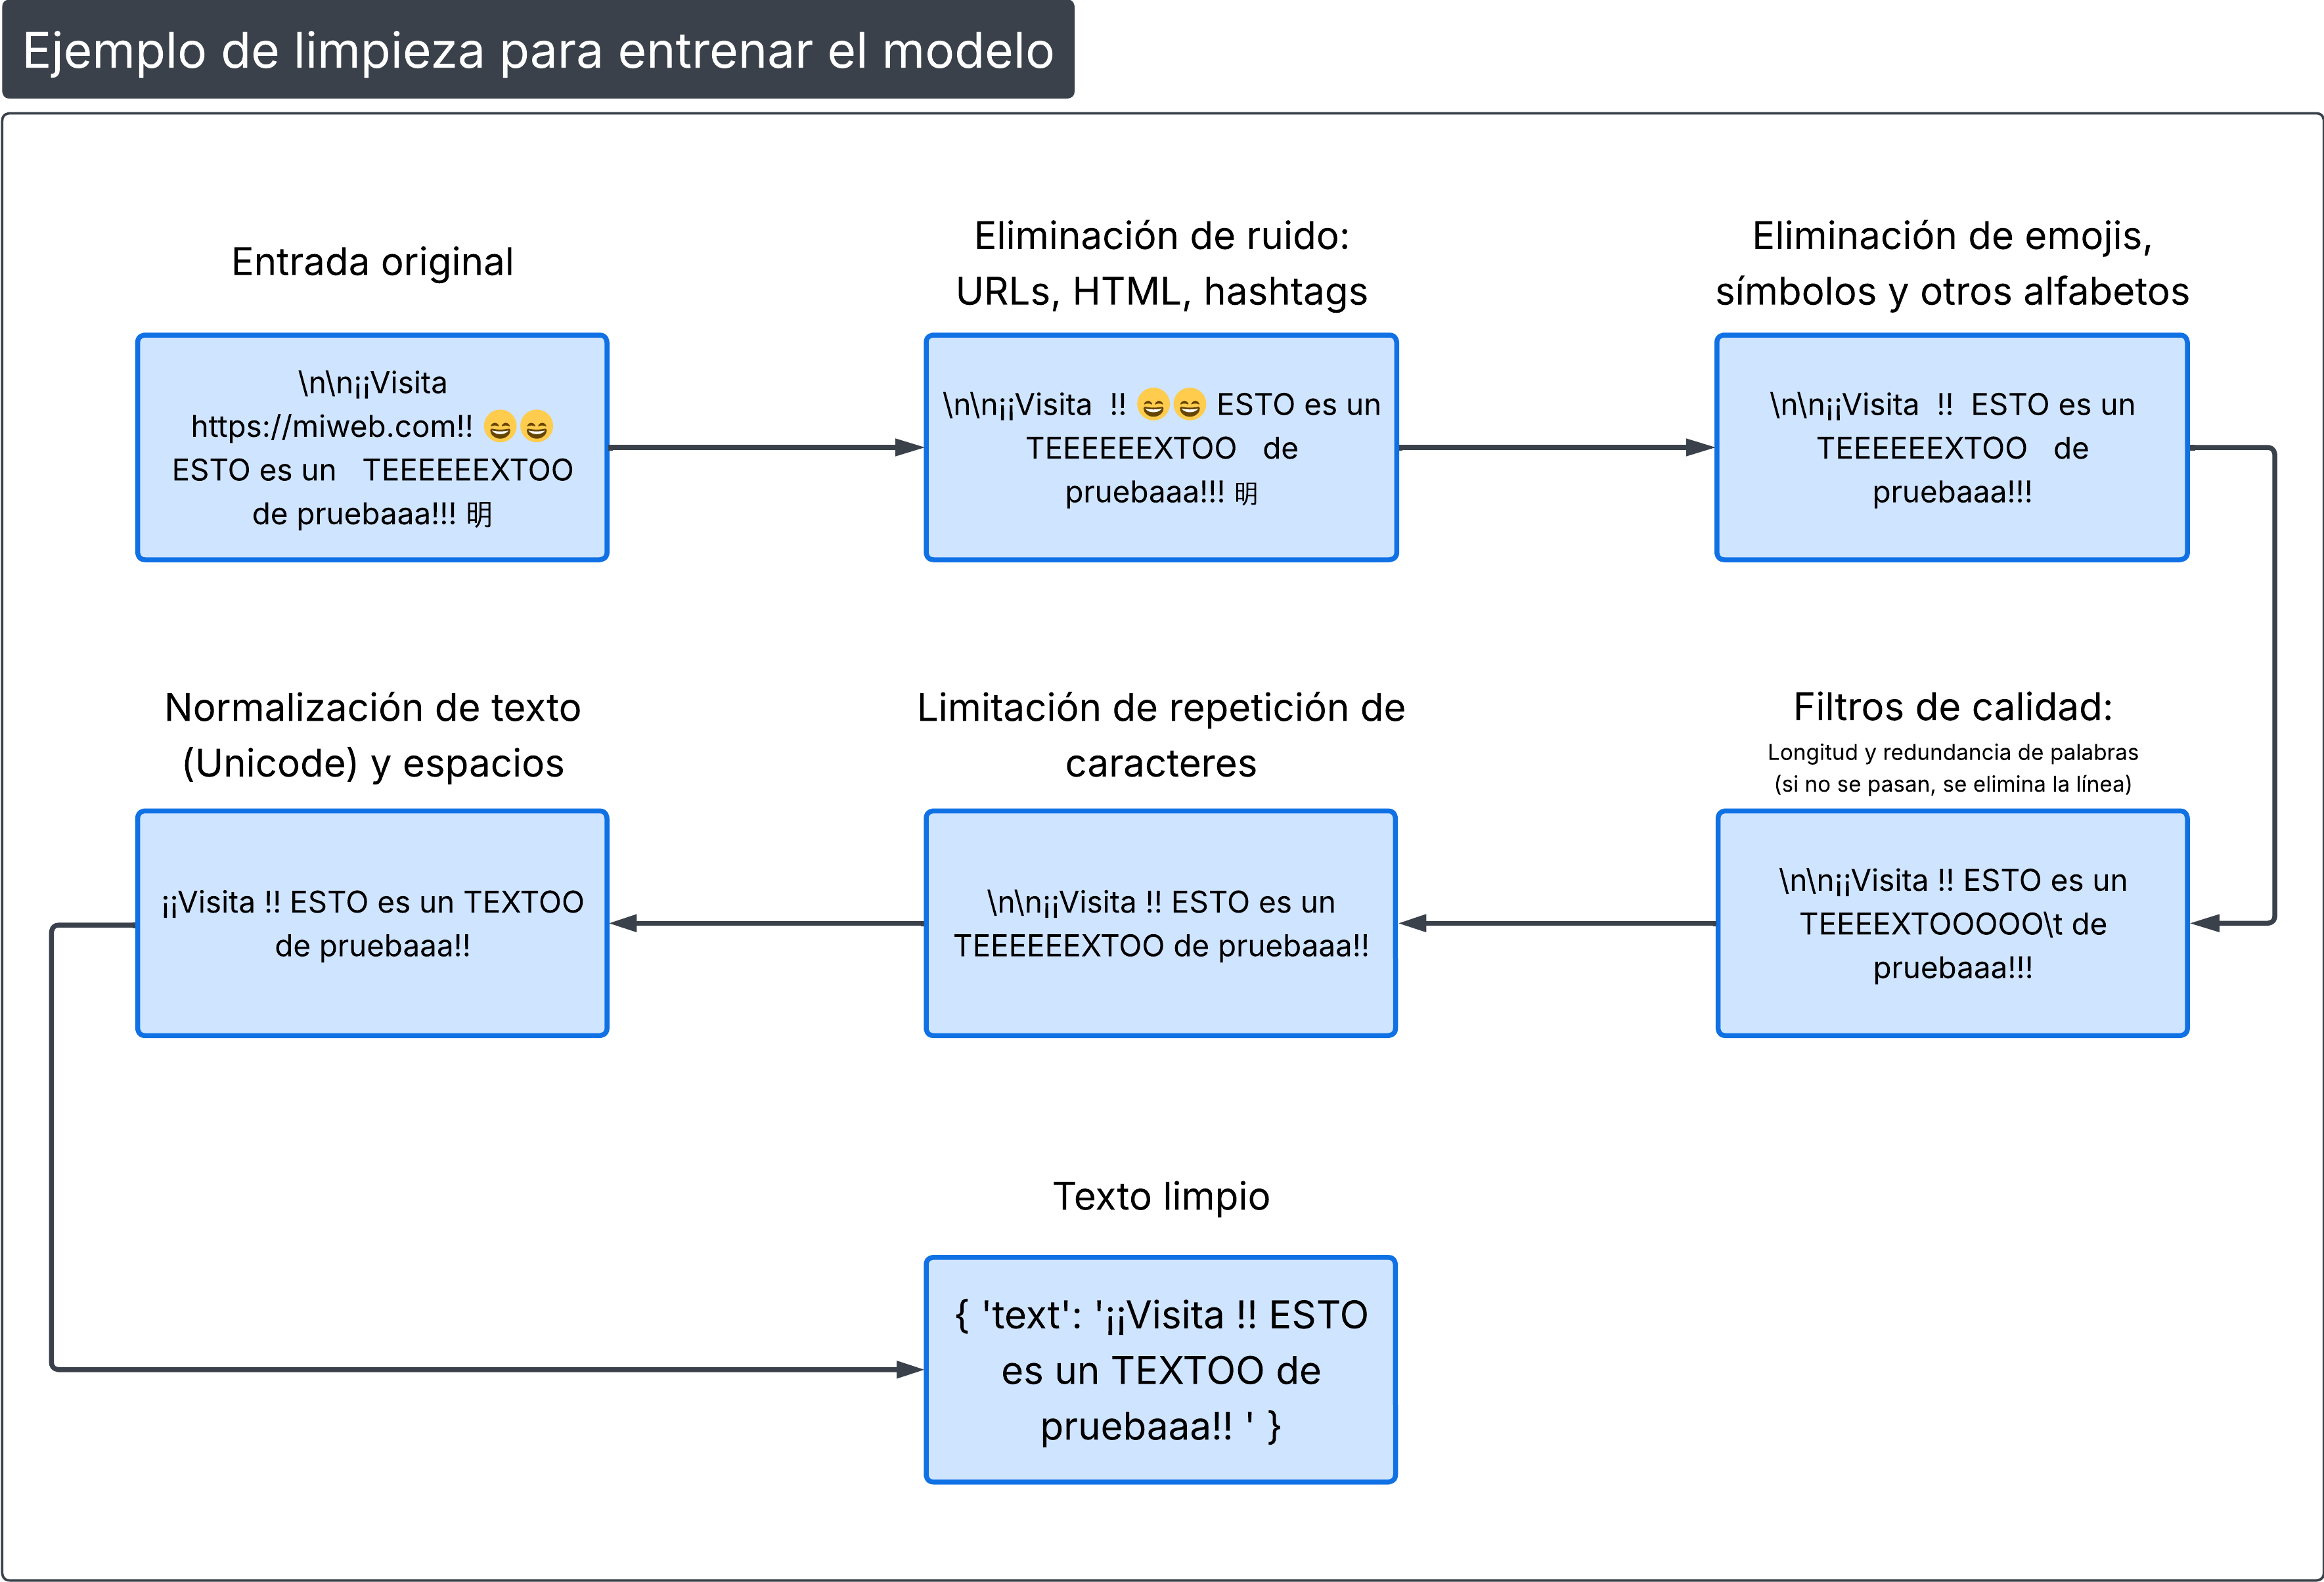
\includegraphics[width=1\textwidth]{figures/DiagramaLimpieza.png}    
    \caption{\label{fig:ejemplo-limpieza} Ejemplo de limpieza de una frase por el sistema. De creación propia.}
\end{figure}

Este proceso de limpieza permite obtener un corpus homogéneo, con una menor cantidad de ruido y adecuado para el análisis comparativo del rendimiento de los modelos de lenguaje seleccionados en lenguas minoritarias.

Aun así, después de analizar el dataset limpio, se observó que, pese a haberse limpiado correctamente, había algunas frases en otras lenguas como el inglés. Esto se debe a que los datasets obtienen mucha información de la web sin filtrarlo manualmente, capturando texto en multiples lenguas. Por eso, se aplicó después de la limpieza un filtro automático de detección de la lengua, con un umbral bajo, evitando borrar incorrectamente frases en la lengua objetivo por fallos en su detección automática, para intentar tener un corpus lo más homogeneo posible.

\subsection{Estadísticas de los datos}
\label{estadisticas-datos}

Tras el análisis de los \nameref{conjuntos-de-datos} disponibles para las tres lenguas objeto de estudio, se seleccionaron dos fuentes principales: el \textit{Corpus NOS} para el gallego y los datos de \textit{NLLB} (Opus) para el asturiano y el aranés. Estas colecciones proporcionan una cobertura amplia y heterogénea, aunque presentan diferencias significativas en longitud media, distribución de tokens y coherencia interna, lo que condicionó las decisiones de preprocesamiento descritas a continuación.

\subsubsection*{Procesamiento inicial y cálculo de estadísticas}

Para cada lengua se calcularon estadísticas de longitud, con el objetivo de caracterizar la distribución real de los datos y determinar valores adecuados de longitud de las muestras durante el entrenamiento. 

\paragraph{Asturiano (datos generales).}

El corpus de NLLB para el asturiano resultó ser el más problemático en términos de longitud. A pesar de contener más de medio millón de líneas, la mayoría eran extremadamente breves. La media fue de 48.14 tokens, la mediana de 42 y el percentil 95 de apenas 100 tokens. El máximo observado fue de 184 tokens y la moda aproximada se situó en torno a los 30 tokens.

\paragraph{Aranés (datos generales).}

El conjunto de datos de NLLB para el aranés contenía un número elevado de textos extremadamente breves. Aunque el corpus no era reducido en número de líneas, la presencia de tantos fragmentos cortos provocaba que el modelo tendiera a cerrar la generación de forma prematura durante las pruebas preliminares. Para intentar mitigar este problema, se aplicó un filtrado mínimo de 40 palabras por muestra, reteniendo únicamente ejemplos con suficiente contenido informativo. La distribución muestra una longitud media de 104.77 tokens, una mediana de 100 y un percentil 95 de 148 tokens. El máximo observado fue de 195 tokens y la moda aproximada se situó en torno a los 90 tokens.

\paragraph{Aranés (instructivo).}

El conjunto instructivo, compuesto por datos generados y pares pregunta–respuesta, presentó una distribución más dispersa y con colas largas. La media alcanzó los 287.15 tokens, con una mediana de 186 y un percentil 95 de 934 tokens. El máximo observado fue de 2\,013 tokens.

\paragraph{Gallego (datos generales).}

Para el gallego se empleó el \textit{Corpus NOS}, del cual se extrajeron fragmentos coherentes procedentes de Wikipedia, prensa, blogs, documentos oficiales y libros disponibles en el dataset. Tras el filtrado por idioma y la limpieza final, el corpus resultante mostró una media de 186.53 tokens, una mediana de 99 y un percentil 95 de 672 tokens. El máximo alcanzó los 5\,966 tokens, reflejando la presencia de textos sustancialmente más largos que en las otras lenguas.

\paragraph{Gallego (instructivo).}

El conjunto instructivo del gallego presentó una media de 311.26 tokens, una mediana de 208 y un percentil 95 cercano a los 983 tokens. El máximo observado fue de 1\,621 tokens.

\subsubsection*{Comparación entre lenguas y entre corpus raw e instructivo}

Las diferencias entre lenguas y entre tipos de corpus son sustanciales y tienen implicaciones directas en el diseño del entrenamiento. Los corpus generales de asturiano y aranés presentan longitudes significativamente menores que el corpus NOS en gallego. 

Los corpus instructivos muestran patrones similares entre lenguas: distribuciones más amplias, colas largas y mayor variabilidad. La media oscila entre 210 y 311 tokens, muy por encima de los corpus generales. Esta diferencia confirma que los instructivos aportan ejemplos más largos y estructurados, esenciales para mejorar la capacidad del modelo para responder preguntas y mantener coherencia en textos extensos.

\subsubsection*{Comparativa de estadísticas entre lenguas}

\begin{longtable}{@{}llrrrrrrr@{}}
\caption{Resumen comparativo de estadísticas de longitud para los corpus generales e instructivos de las tres lenguas.}
\label{tab:estadisticas_globales} \\
\toprule
Lengua & Tipo & Media & Mediana & P95 & P98 & Máx. & Mín. & Moda \\ 
\midrule
\endfirsthead

\multicolumn{9}{c}{\tablename\ \thetable{} -- continuación} \\
\toprule
Lengua & Tipo & Media & Mediana & P95 & P98 & Máx. & Mín. & Moda \\ 
\midrule
\endhead

\midrule \multicolumn{9}{r}{Continúa en la siguiente página} \\
\endfoot

\bottomrule
\endlastfoot

Asturiano & General & 48.14 & 42 & 100 & 120 & 184 & 6 & 30 \\
Asturiano & Instructivo & 210.13 & 112 & 740.9 & 910.8 & 1453 & 20 & 40 \\

Aranés & General & 104.77 & 100 & 148 & 159 & 195 & 57 & 90 \\
Aranés & Instructivo & 287.15 & 186 & 934 & 1101 & 2013 & 26 & 50 \\

Gallego & General & 186.53 & 99 & 672 & 1087.08 & 5966 & 28 & 70 \\
Gallego & Instructivo & 311.26 & 208 & 982.7 & 1151.8 & 1621 & 19 & 30 \\

\end{longtable}

\begin{figure}[H]
    \centering
    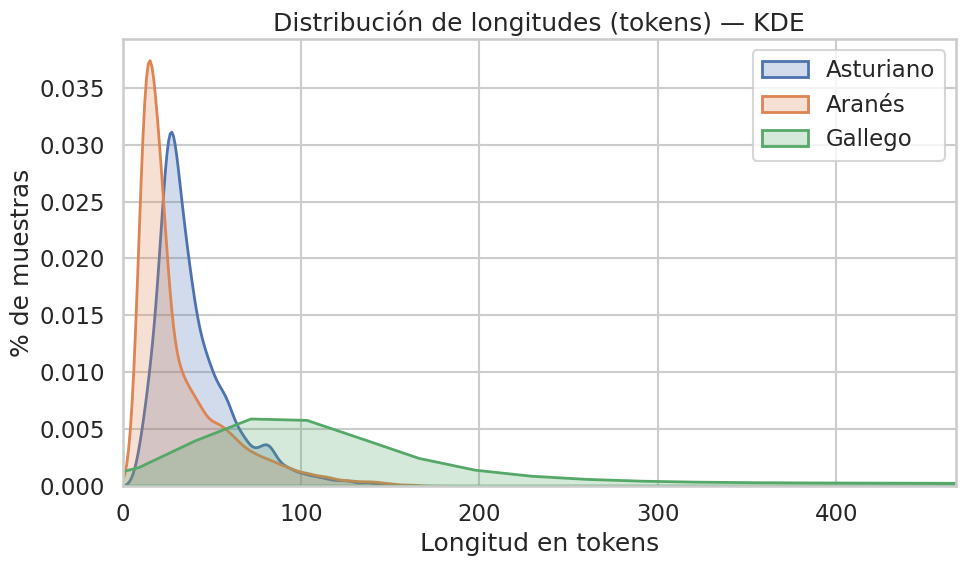
\includegraphics[width=0.8\textwidth]{figures/KDE_DistribucionLongitudTokensARNOriginal.png}    
    \caption{\label{fig:distribucion-longitudes-arn-original}Distribución de longitud de las muestras por lengua en los datasets originales. De creación propia.}
\end{figure}

Como se puede ver en la Figura \ref{fig:distribucion-longitudes-arn-original}, el Aranés tiene la mayoría de muestras demasiado pequeñas y se ha visto que afecta al entrenamiento. Por lo que se ha filtrado a 40 el mínimo de palabras en las muestras del dataset de entrenamiento del aranés, cambiando su distribución como se puede observar en la siguiente Figura \ref{fig:distribucion-longitudes}. También se puede ver como el dataset del gallego es de mucha mejor calidad, con unas muestras con longitudes mucho más distribuidas. Ambas estadísticas son con los datasets ya limpios y filtrados.

\begin{figure}[H]
    \centering
    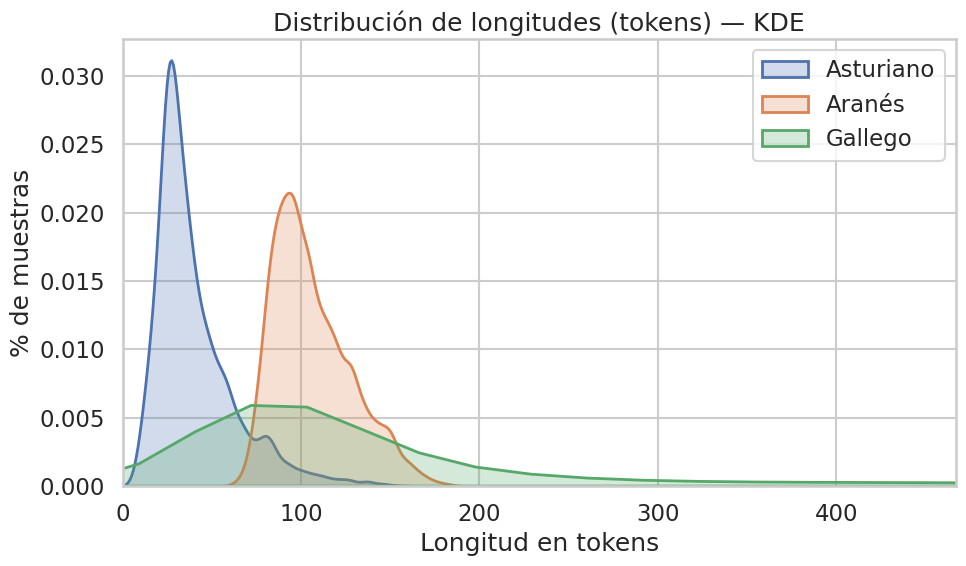
\includegraphics[width=0.8\textwidth]{figures/KDE_DistribucionLongitudTokens.png}    
    \caption{\label{fig:distribucion-longitudes}Distribución de longitud de las muestras por lengua en los datos de entrenamiento. De creación propia.}
\end{figure}



\subsection{Implicaciones para el entrenamiento}

Las diferencias entre lenguas y tipos de corpus condicionaron directamente el diseño del conjunto de entrenamiento. En el caso del asturiano y el aranés, la abundancia de textos breves obligó a aplicar filtrados mínimos y a seleccionar cuidadosamente el valor de \texttt{max\_length}, mientras que en el gallego fue necesario controlar la presencia de textos extremadamente largos para evitar desbordamientos de memoria durante el entrenamiento.

El uso de datos instructivos permitió complementar los corpus generales con ejemplos más largos y estructurados, mejorando la capacidad del modelo para responder preguntas y mantener coherencia en textos extensos. Esta estrategia resultó especialmente útil en lenguas con corpus generales muy breves, como el asturiano.

\subsection{Datos instructivos y generación sintética}
\label{datos-instructivos}

El entrenamiento de un modelo en modo \textit{Causal LM} (Modelado de Lenguaje Causal) permite que este aprenda la distribución de probabilidad de los nuevos tokens respecto a su contexto. Sin embargo, esta aproximación por sí sola no garantiza que el modelo adquiera la capacidad de interactuar de forma directa con un usuario, responder preguntas de manera coherente o asimilar un formato puramente instructivo. 

Para mitigar esta limitación y guiar al modelo hacia un comportamiento de asistente, se diseñó un flujo de trabajo para la obtención de un conjunto de datos instructivos sintéticos. Como modelo generador principal se empleó el modelo de gran tamaño \textit{GPT-OSS 120B} a través de la API de Groq, tomando como base oraciones breves extraídas del corpus de \textit{Tatoeba} para las tres lenguas de bajos recursos objeto de estudio: asturiano, gallego y aranés. 

Con el propósito de dotar de una mayor diversidad al corpus y exponer al modelo a secuencias de texto más largas dentro de las restricciones impuestas por la VRAM disponible, la generación automatizada se dividió en dos estrategias diferenciadas mediante ingeniería de instrucciones (\textit{prompt engineering}):

\begin{itemize}
    \item \textbf{Transformación y ampliación de textos:} Esta estrategia entrena al modelo en tareas de reescritura y expansión lingüística. Se utilizaron plantillas que exigían al modelo generador realizar diferentes tareas a partir de una oración de Tatoeba: desarrollar el contenido añadiendo detalles, dar consejos, cambiar el registro a formal o informal, o parafrasear la información. 
    
    Para facilitar el procesamiento de las respuestas del modelo a nivel de código, se forzó al generador a encapsular su salida bajo etiquetas XML (\texttt{<respuesta>...</respuesta>}), facilitando su posterior estructuración en el formato de turnos conversacionales utilizado en el ajuste fino.
    
    A continuación, se ilustra el resultado de este proceso con un ejemplo real extraído del corpus generado para el asturiano:
    
    \begin{quotation}
        \noindent\textbf{Texto base (Tatoeba):} \textit{Tas buenu pa dir a nengún sitiu.}\\
        \textbf{Instrucción aplicada:} \textit{Da un conseyu relacionáu con esti conteníu:}\\
        
        \noindent\textbf{Formato estructurado final:}
       \begin{verbatim}
<​|user|>
Da un conseyu relacionáu con esti conteníu:
Tas buenu pa dir a nengún sitiu.
<​|assistant|>
Si sientes que tas buenu pa dir a nengún sitiu, ye importante 
reflexonar sobre a quién quies dir la mensaxe y por qué. Escueyi 
un destinatariu concretu, adapta'l tonu al so públicu y sé claru 
col conteníu. Así, la comunicación será más eficaz y evites 
perder oportunidaes por hablar en llugar que nun tien audiencia.
\end{verbatim}
    \end{quotation}

    \item \textbf{Comprensión lectora (Pregunta - Respuesta):} Orientada a dotar al modelo de la capacidad de extracción de información y síntesis precisa. Mediante plantillas específicas (\textit{QA Templates}), se suministró un texto base al modelo generador con la instrucción de formular una pregunta lógica y directa sobre el mismo, acompañada de su respectiva respuesta detallada. El formato de salida de la API se restringió estrictamente mediante bloques diferenciados (\texttt{<pregunta>} y \texttt{<respuesta>}).
    
    Un ejemplo representativo del resultado de esta estrategia, también sobre el corpus en asturiano, se detalla a continuación:

    \begin{quotation}
        \noindent\textbf{Texto base (Tatoeba):} \textit{El cielu del atapecer ye roxu.}\\
        \textbf{Instrucción aplicada:} \textit{Inventa una pregunta sencilla sobre esti fragmentu y da una respuesta curtia pero natural.}\\
        
        \noindent\textbf{Formato estructurado final:}
        \begin{verbatim}
<|user|>
¿Por qué'l cielu del atapecer ye roxu?
<|assistant|>
Porque la dispersión de la lluz del Sol pola atmósfera fai que la 
lluz azul se disperse y solo quede la lluz roja visible.
        \end{verbatim}
    \end{quotation}
\end{itemize}

Los conjuntos de datos que se han generado y utilizado para el entrenamiento se encuentran disponibles en HuggingFace con el resto de materiales del TFG \url{https://hf.co/collections/MiguelGP-13/tfg} \cite{lexicons_2025, galician_instructive_2025, asturian_instructive_2025, aranes_instructive_2025, asturian_annotated_2025, galician_annotated_2025, aranes_annotated_2025, asturian_cloze_2025, galician_cloze_2025, aranes_cloze_2025}.

\subsubsection{Robustez del flujo y control de calidad}
Debido a que las respuestas de los modelos de lenguaje pueden sufrir alucinaciones de formato o errores de truncado en la API, el script implementado en Python incorporó filtros heurísticos automatizados de validación. Tras cada llamada al modelo, el sistema verifica la presencia íntegra de las etiquetas delimitadoras requeridas y comprueba que la longitud de los textos generados cumpliera con unos umbrales mínimos de calidad. 

Dado que el objetivo metodológico consistía en equilibrar estrictamente el volumen de datos por lengua y tarea, se adoptó un enfoque de ejecución por cuotas. El algoritmo descartaba de manera transparente cualquier salida defectuosa o mal formateada y continuaba realizando peticiones de forma iterativa hasta asegurar un total exacto de $N=500$ ejemplos instructivos válidos y limpios para cada uno de los subconjuntos, garantizando así la homogeneidad del corpus final de entrenamiento.


\section{Preparación del modelo}

Tras la evaluación de distintos modelos base, se seleccionó \textbf{Qwen-2.5 7B} cuantizado a 4 bits como punto de partida para este trabajo. Esta elección se debe a que ofrece un equilibrio adecuado entre capacidad de comprensión, calidad generativa y conocimiento de las lenguas de estudio, como puede verse en los \nameref{ch:Resultados base}.

\subsection{Capas del Lora}

Se ha decidido aplicar los adaptadores LoRA  específicamente sobre las capas de atención (\texttt{q\_proj}, \texttt{k\_proj}, \texttt{v\_proj}), la capa Output Projection (\texttt{o\_proj}), encargada de combinar la información de todas las cabezas de atención y proyectarla de vuelta al tamaño original del modelo, y las capas de la etapa de feed forward (\texttt{gate\_proj}, \texttt{up\_proj} y  \texttt{down\_proj}) del Transformer.
La selección de estas capas responde a criterios tanto teóricos como empíricos. Por un lado, las proyecciones de atención constituyen el núcleo del mecanismo de atención, responsable de modelar las relaciones contextuales entre los elementos de una secuencia. Modificar estas matrices permite ajustar de manera directa cómo el modelo interpreta y pondera la información lingüística.

Por otro lado, las capas del MLP son las encargadas de transformar las representaciones internas y aportar capacidad expresiva adicional. Estudios previos sobre adaptadores, como AdapterFusion \cite{pfeiffer2021adapterfusionnondestructivetaskcomposition}, muestran que insertar módulos entrenables en estas capas permite modificar el comportamiento del modelo sin alterar los pesos originales, manteniendo así la integridad del modelo base y evitando efectos destructivos.

\subsection{Configuración inicial de hiperparámetros}

La configuración de hiperparámetros es un componente esencial en el proceso de entrenamiento, especialmente en contextos con recursos computacionales limitados y cuando se emplean técnicas como QLoRA. El Cuadro \ref{tab:hiperparametros_iniciales} resume los parámetros principales y los valores seleccionados.

\begin{table}[H]
\centering
\begin{tabular}{l l}
\hline
\textbf{Hiperparámetro} & \textbf{Valor} \\
\hline
Rango LoRA (\texttt{r}) & 8 \\
Alpha & 16 \\
Dropout & 0.1 \\
Batch size & 2 \\
Épocas de entrenamiento & 2 \\
Learning rate & 1e-4 \\
Scheduler & Cosine \\
Warmup ratio & 0.1 \\
Optimizador & Paged AdamW 32-bit \\
\hline
\end{tabular}
\caption{Hiperparámetros iniciales.}
\label{tab:hiperparametros_iniciales}
\end{table}

\subsubsection{Parámetros de LoRA}

\paragraph{Rango (\texttt{r} = 8).}
El rango determina la dimensionalidad interna de los adaptadores LoRA. Un valor de 8 proporciona un equilibrio adecuado entre capacidad de adaptación y eficiencia computacional. Valores mayores permiten aprender representaciones más complejas, pero incrementan el número de parámetros entrenables y el riesgo de sobreajuste, especialmente en escenarios de bajo recurso como este.

\paragraph{Alpha = 16.}
Este parámetro actúa como un factor de escalado que controla la contribución de los adaptadores respecto al modelo base. Un valor moderado como 16 permite una adaptación estable sin introducir oscilaciones excesivas en el gradiente.

\paragraph{Dropout = 0.1.}
Se introduce un pequeño dropout para reducir el sobreajuste. Dado que el corpus es relativamente reducido y homogéneo, este valor ayuda a mejorar la generalización sin afectar negativamente a la estabilidad del entrenamiento.

\subsubsection{Parámetros de entrenamiento}

\paragraph{Batch size = 1 y Gradient Accumulation = 2.}
Las limitaciones de memoria de la GPU impiden utilizar batch sizes mayores. Para compensarlo, se acumulan gradientes durante dos pasos, obteniendo un batch efectivo de tamaño 2. Esto mejora la estabilidad del entrenamiento sin incrementar el uso de memoria.

\paragraph{Learning rate = 1e-4.}
Los modelos adaptados mediante LoRA toleran tasas de aprendizaje más altas que los modelos entrenados desde cero. 

\paragraph{Épocas = 2.}
El número de épocas se mantiene bajo debido al coste computacional del entrenamiento y al riesgo de sobreajuste en un corpus pequeño.

\subsubsection{Scheduler, warmup y optimizador}

\paragraph{Scheduler cosenoidal.}
El scheduler cosenoidal reduce progresivamente la tasa de aprendizaje, favoreciendo una convergencia más suave y estable. Este tipo de scheduler es especialmente útil en entrenamientos cortos, donde los cambios bruscos pueden afectar negativamente al rendimiento.

\paragraph{Warmup ratio = 0.1.}
Durante el 10\% inicial del entrenamiento, la tasa de aprendizaje aumenta gradualmente. Esto evita picos de gradiente al inicio, que son especialmente problemáticos en modelos cuantizados y con adaptadores LoRA.

\paragraph{Paged AdamW 32-bit.}
Este optimizador está diseñado específicamente para QLoRA, gestionando eficientemente los pesos cuantizados y reduciendo el uso de memoria mediante paginación.


\section{Entrenamiento del modelo}

Para definir la mejor manera de entrenar, se han realizado pruebas iniciales con el asturiano, y luego se han probado la mejor metodología encontrada en el aranés y el gallego, adaptándose a los corpus de cada lengua y analizando los resultados.

Los modelos entrenados en todas las lenguas y con todas las configuraciones se encuentran disponibles en HuggingFace con el resto de materiales del TFG \url{https://hf.co/collections/MiguelGP-13/tfg} \cite{asturian_lora_2025, asturian_concat_2025, asturian_concat_instructive_2025, galician_lora_2025, aranes_lora_2025, aranes_lora_instructive_2025}.

\subsection{Optimización de la longitud de las muestras}
\label{problemas-longitud-muestra}

Los primeros experimentos de entrenamiento se realizaron utilizando una versión tokenizada del corpus con una longitud fija de 512 tokens por muestra. Esta decisión inicial, aunque habitual en muchos flujos de trabajo, resultó poco adecuada para nuestros datos, ya que tras analizar el conjunto de datos, se observó que la longitud media de las frases era cercana a los 50 tokens, lo que implicaba que la mayor parte de cada entrada estaba compuesta por \textit{padding}. Como consecuencia, el modelo aprendió que el token más frecuente era el token de fin de secuencia, produciendo respuestas vacías o extremadamente breves. 

Para solucionar esto, en vez de poner una longitud definida de los datos, se investigó emplear el percentil 95 o 98 de la cantidad de tokens por frase como referencia para determinar la longitud máxima razonable, evitando tanto el truncado excesivo como la inclusión de demasiado padding. Además se vió que por limitaciones de cómputo, el máximo absoluto por muestra es de 160 tokens, ya que si las secuencias son más largas, el servidor devolvía OoME (Out of Memory Error), es decir, que la tarjeta gráfica no tiene más espacio en la memoria VRAM.


Una vez ajustada la longitud máxima a valores más acordes con la distribución real del corpus, el modelo comenzó a generar texto de forma más consistente. Aun así, continuaba produciendo \textbf{respuestas cortas o incompletas}. Como aspecto positivo, al evaluar estos primeros modelos se observó que, pese a su baja fluidez, mostraban una mejora apreciable en tareas de corrección ortográfica y morfológica. Esto sugiere que el modelo sí estaba captando patrones lingüísticos relevantes, aunque todavía no era capaz de producir textos extensos o naturales.

La única solución real para mitigar este problema es tener muestras más largas. Para ello, se probó a \textbf{concatenar varias frases del dataset en una}, aumentando la longitud efectiva de las muestras y proporcionando al modelo contextos más ricos y coherentes. Sin embargo, esta aproximación tiene dos problemas. El primero y menos importante para este estudio, es que reduce el número de muestras diponibles aun más en un dataset ya bastante reducido. Debido a la capacidad de cómputo disponble, no se va a poder entrenar sobre el dataset entero, por lo que este problema no afectaría al proyecto. El segundo problema y más importante, es que al concatenar frases que no tienen por que tener nada que ver entre sí, se ha visto que hace que el modelo pierda conocimiento de como generar texto de manera coherente, mezclando frases una detrás de otra sin tener siempre conexión entre ellas. Para conseguir textos más largos, coherentes y de mayor variedad temática, se contactó con la \textbf{Academia de la Llingua Asturiana} \cite{ALLA2024}, para solicitar el uso de los artículos y publicaciones de sus revistas digitales. Hasta el momento de entrega de este TFG no se ha recibido respuesta.

 Después de aplicar el cambio de concatenar muestras del conjunto de datos y corrección de la longitud de las muestras, el modelo empezó a generar textos más largos en asturiano, pero perdió bastante coherencia, por lo que empezó a responder las preguntas peor. 
 
 Para intentar evitarlo, se ha decidido probar a hacer un entrenamiento final con \nameref{datos-instructivos} con prompt y respuesta coherentes al modelo concatenado generados automáticamente.
 
\subsection{Optimización de hiperparámetros}
 No se han observado grandes variaciones al optimizar los hiperparámetros. Se optó por reducir la tasa de aprendizaje (\textit{learning rate}) e incrementar la acumulación de gradientes (\textit{gradient accumulation}). El objetivo de esta configuración es mitigar el sobreajuste (\textit{overfitting}) del conjunto de datos y evitar actualizaciones de pesos excesivamente abruptas que puedan derivar en el fenómeno de olvido catastrófico \cite{luo2023an}. 
 
\subsection{Análisis cualitativo de las pruebas en asturiano}
Los ejemplos cualitativos tanto del asturiano como de las otras lenguas se encuentran en los \nameref{resultados_cualitativos_qlora}.
En los ejemplos cualitativos se puede ver como el concatenado escribe respuestas mucho más extensas y ricas, pero cambiando completamente de tema repentinamente, mientras que el modelo entrenado con frases más cortas es más conciso, a veces demasiado.

En estos y otros ejemplos, se observó que el modelo generaba con bastante frecuencia sobre temas muy específicos, como aspectos políticos, legales o historia. Esto probablemente se debe a la alta prevalencia en el dataset de estos temas y se estudiará como se comportan los modelos en las otras lenguas.

 \subsection{Metodología para aranés y gallego}
 Con los resultados obtenidos de las pruebas del asturiano, se va a entrenar los modelos en las otras lenguas. 
 Se ha visto que concatenar no aporta valor, por lo que se entrenará con los textos más largos encontrados en el dataset, pero sin concatenar muestras. Se cortarán los datos al percentil 95 del dataset y posteriormente, cuando el modelo haya aprendido la lengua, si el modelo ha perdido cohesión en la generación, se entrenará con los datasets sintéticos instructivos para obligar al modelo a seguir mejor el estilo y no acabar las respuestas demasiado pronto.

 \subsubsection{Aranés}
 El conjunto de datos del Aranés tiene muchas muestras muy cortas, con una mediana de 22 tokens y una moda de 10 tokens. Por lo que al entrenar, tenía el mismo problema que el asturiano, generando texto muy corto. El problema es que si le fuerzas a sacar un mínimo de tokens, en vez de generar texto como el modelo de asturiano, generaba puntos, queriendo acabar las frases desde el principio. Por lo que como diferencia con los otros dos modelos, se filtró su dataset cogiendo las muestras con mínimo 40 palabras. Esto redujo mucho el tamaño del dataset y enseña al modelo a generar siempre contenido largo, lo cual tampoco es perfecto, pero si mejor que que no genere nada. En los resultados de la sección \ref{tab:metricas_calidad_lengua_Aranés} se puede ver que consigue que el modelo genere texto, pero de peor calidad.

 \subsubsection{Gallego}
El gallego, como lengua oficial de Galicia, pese a ser una lengua minoritaria, tiene una cantidad de datos disponibles mucho mayor, haciendo posible un entrenamiento mejor con una longitud media de las muestras y una variedad temática mayor. Por esta disponibilidad de datos de mayor calidad, el modelo solo se ha entrenado con muestras seleccionadas, sin concatenar ni necesitar los datos instructivos generados.
Los datos al contrario que en las otras dos lenguas, venían en documentos largos en vez de directamente en frases. Esto permite coger muestras coherentes y cohesionadas sin importar la longitud, dando un entrenamiento mucho mejor.

\subsection{Longitud de entrenamiento y dinámica de la función de pérdida}
\label{subsec:longitud_entrenamiento}

En la Figura \ref{fig:comparativa-loss} se analiza la evolución de la función de pérdida (\textit{loss}) a lo largo de los pasos de entrenamiento para los distintos modelos. En el contexto del \textit{fine-tuning} mediante QLoRA usando Casual LLM, el \textit{loss} utilizado es la entropía cruzada (\textit{cross-entropy loss}) \cite{vaswani2023attentionneed}. Esta métrica cuantifica la discrepancia entre la distribución de probabilidad predicha por el modelo para el siguiente \textit{token} y el \textit{token} real (\textit{ground truth}) del texto de entrenamiento. Por tanto, su medición y evolución temporal son indicadores críticos de la convergencia del modelo: un descenso sostenido demuestra que la red está optimizando sus adaptadores de bajo rango para capturar los patrones lingüísticos y semánticos del nuevo corpus.

\begin{figure}[H]
    \centering
    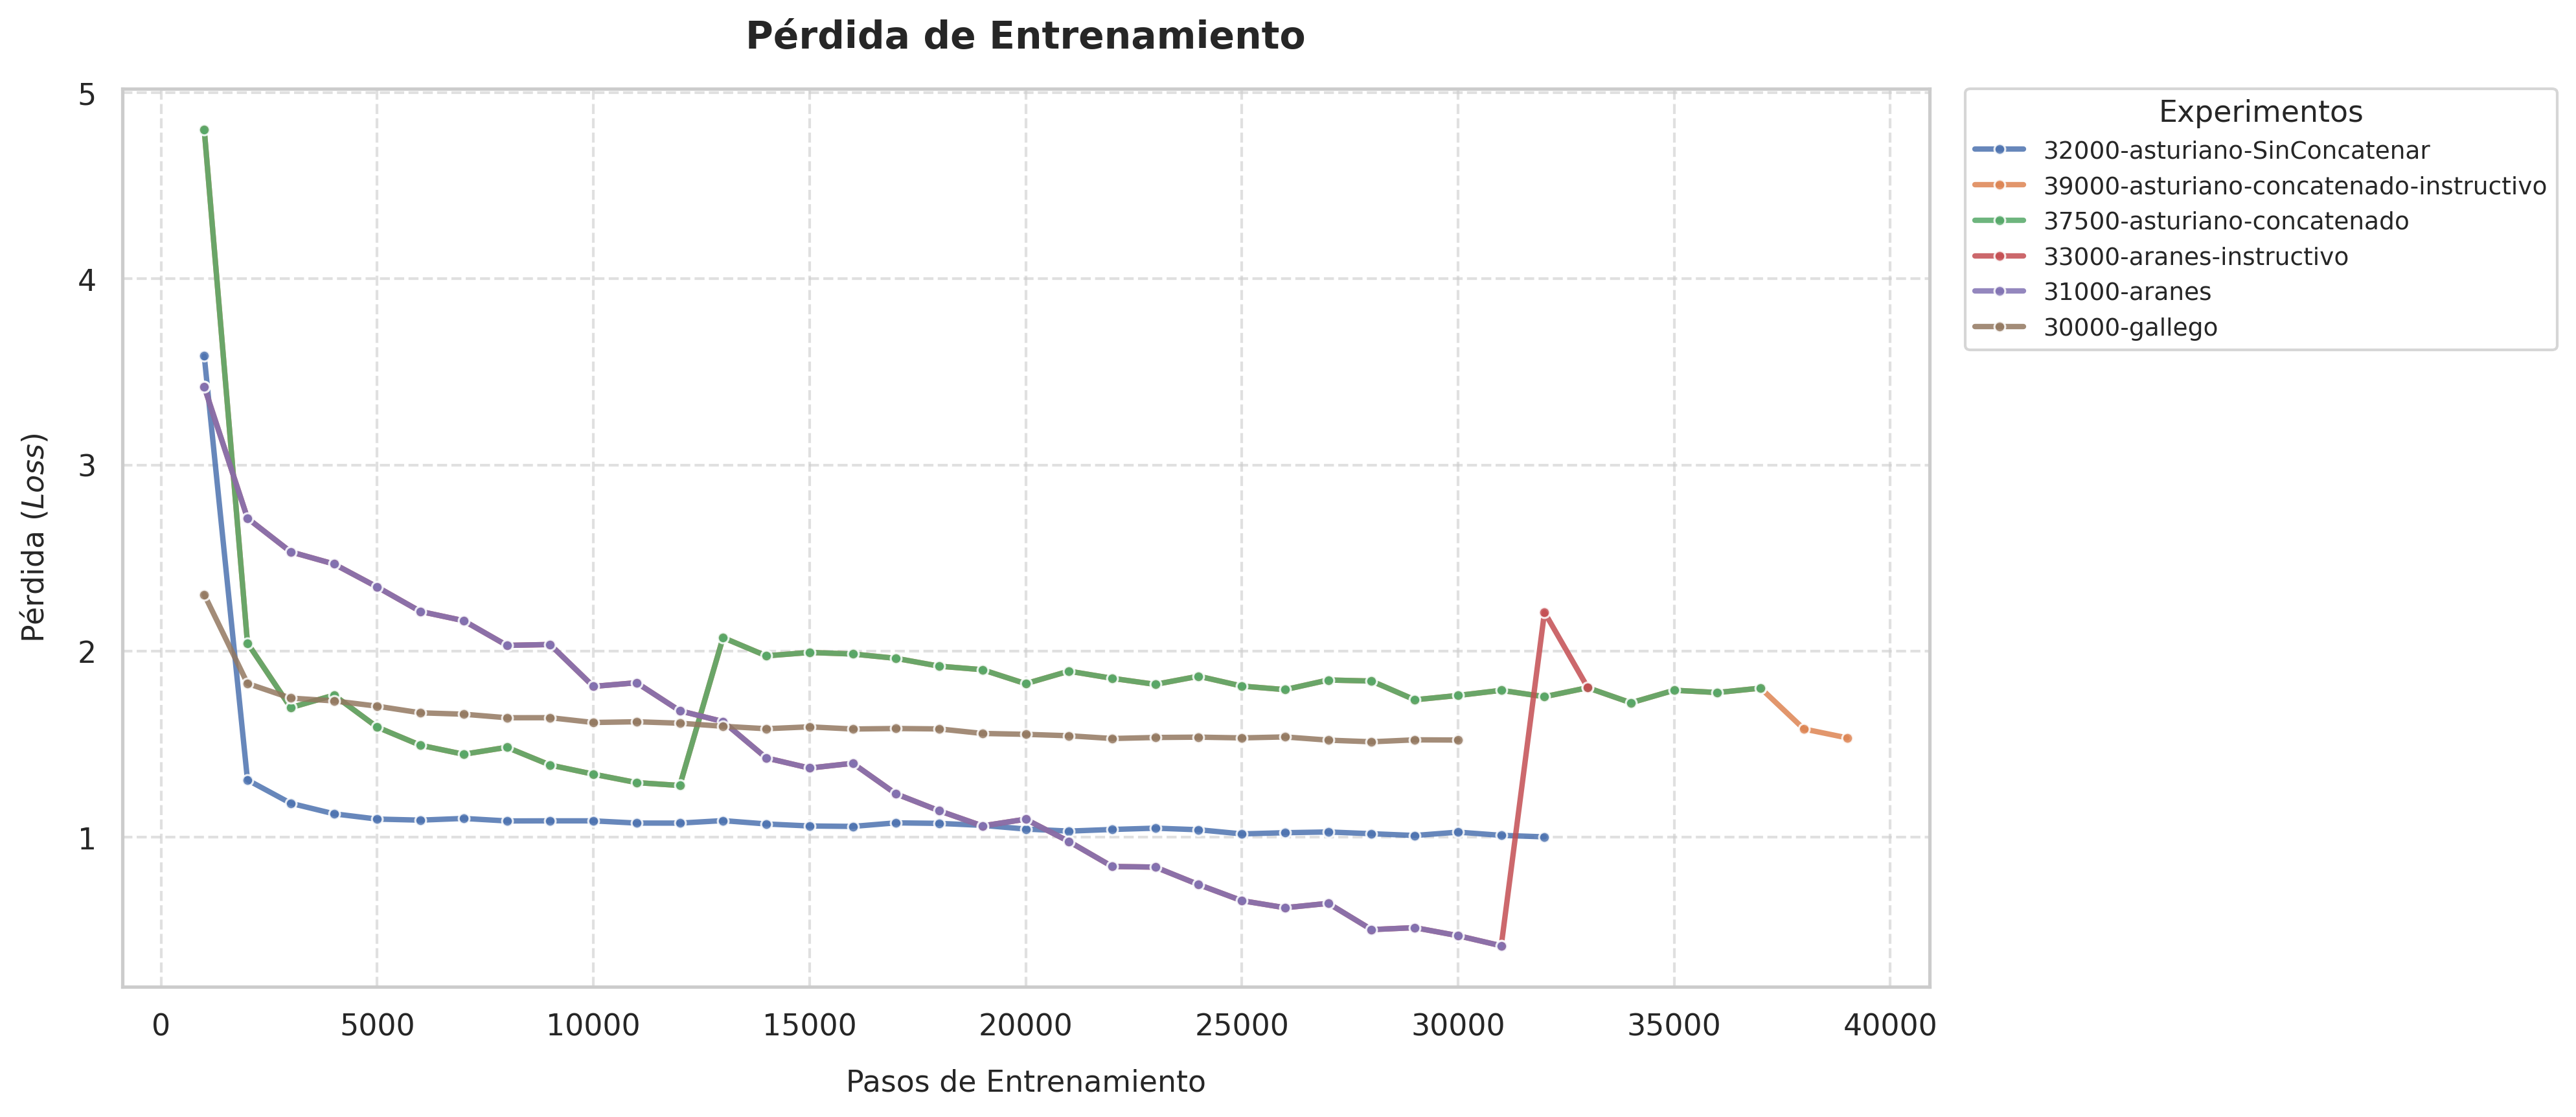
\includegraphics[width=1\textwidth]{figures/comparativa_loss.png}    
    \caption{Comparativa de funciones de pérdida de entrenamiento. De creación propia.}
    \label{fig:comparativa-loss}
\end{figure}

A partir de las curvas obtenidas, se observa que los entrenamientos del modelo para el gallego y el asturiano sin concatenar presentan las dinámicas más estables. El modelo de gallego estabiliza su pérdida en un valor ligeramente más alto, un comportamiento esperado debido a la alta variedad y riqueza del conjunto de datos utilizado, lo que dificulta que la entropía cruzada llegue a valores cercanos a cero pero garantiza una mayor capacidad de generalización.

Por su parte, el modelo del aranés es el que presenta el descenso de pérdida más rápido. Al tratarse del conjunto de datos más reducido, esta abrupta caída sugiere que el modelo sufría un leve sobreajuste (\textit{overfitting}), memorizando las secuencias en lugar de aprender sus estructuras subyacentes. Esto explica por qué, al cambiar los datos al modo instructivo en fases posteriores, el \textit{loss} inicial se eleva de manera tan notable ante la introducción de formatos no vistos.

Por último, el modelo asturiano concatenado muestra la curva más inestable y alta, lo cual se atribuye a que las muestras concatenadas de forma contigua introducen rupturas de contexto que resultan caóticas para el modelado de lenguaje causal. Sin embargo, se constata que la posterior introducción de las muestras instructivas, significativamente más estructuradas y delimitadas, corrige esta tendencia inestable, permitiendo una optimización más eficiente y mejorando el rendimiento general del entrenamiento.